% dvisvgm --pdf name
% latexmk -C
\documentclass[preview]{standalone}
\usepackage{tikz}
\usepackage{amsmath}
\usepackage{color}
\usepackage{tabularray}
\definecolor{Sushi}{rgb}{0.545,0.756,0.294}
\definecolor{Frost}{rgb}{0.933,0.968,0.89}
\usetikzlibrary{shapes.geometric, arrows}
\tikzstyle{block} = [rectangle, rounded corners,
minimum width=3.5cm,
minimum height=2cm,
text centered, 
draw=gray]

\tikzstyle{io} = [trapezium, 
trapezium stretches=true,
trapezium left angle=70, 
trapezium right angle=110, 
minimum width=3.5cm, 
minimum height=2cm, text centered, 
draw=gray]

\tikzstyle{process} = [rectangle, 
minimum width=3.5cm,
minimum height=2cm,
text centered, 
text width=3cm, 
draw=gray]

\tikzstyle{decision} = [diamond, 
minimum width=3cm, 
minimum height=1cm, 
text centered, 
draw=gray]
\tikzstyle{arrow} = [thick,->,>=stealth]

\tikzstyle{circle} = [circle, 
minimum size=1cm, 
text centered, 
draw=gray]

\begin{document}
    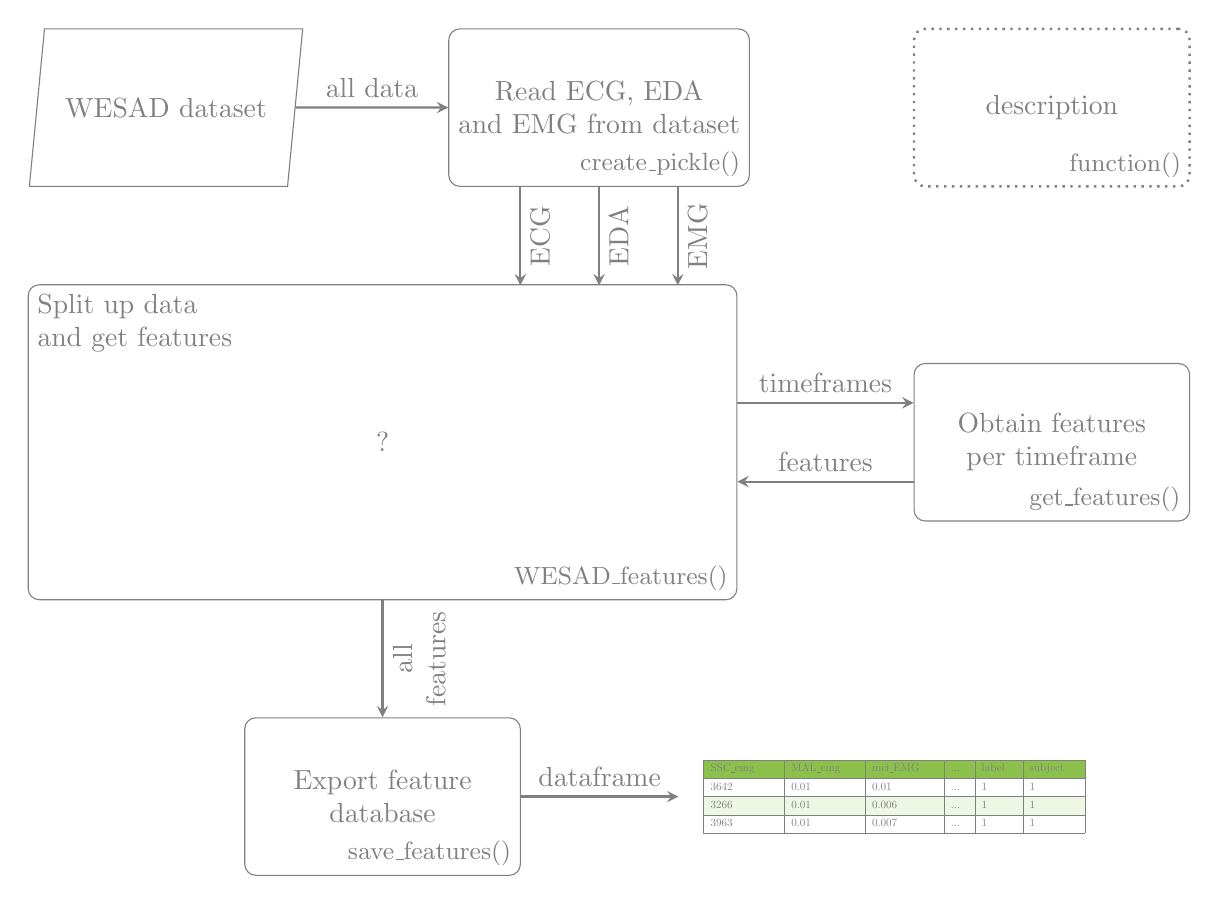
\begin{tikzpicture}[transform shape, every node/.append style={}, color=gray, node distance = 3.5cm]
        % All blocks
        \node (WESAD) [io] {WESAD dataset};

        \node (read_WESAD) [block, right of=WESAD, xshift = 2 cm, align =center] {Read ECG, EDA \\ and EMG from dataset};
        \node at (read_WESAD.south east) [anchor = south east] {\small create\_pickle()};

        \node (wesad_features) [block, below of = read_WESAD, minimum width = 9 cm, minimum height = 4 cm, xshift = -2.75 cm, yshift = -0.75 cm] {?};
        \node at (wesad_features.south east) [anchor = south east] {\small WESAD\_features()};
        \node at (wesad_features.north west) [anchor = north west, align =left ] {Split up data \\ and get features};

        \node (get_features) [block, right of = wesad_features, xshift = 5 cm, align= center] {Obtain features \\ per timeframe};
        \node at (get_features.south east) [anchor = south east] {\small get\_features()};

        \node (save_features) [block, below of = wesad_features, yshift = -1 cm, align =center] {Export feature \\ database};
        \node at (save_features.south east) [anchor = south east] {\small save\_features()};

        \node (legend) [block, right of = read_WESAD, xshift = 2.25 cm, dotted, line width = 0.3mm, align = left] {description};
        \node at (legend.south east) [anchor = south east] {\small function()};

        % WESAD to read_WESAD
        \draw [arrow] (WESAD) -- node[midway, above] {all data} (read_WESAD);

        % All around WESAD_features
        \draw [arrow] ([xshift=-1cm]read_WESAD.south) -- node[midway, rotate=90, below] {ECG} +(0, -1.25);
        \draw [arrow] (read_WESAD.south) -- node[midway, rotate=90, below] {EDA} +(0, -1.25);
        \draw [arrow] ([xshift=1cm]read_WESAD.south) -- node[midway, rotate=90, below] {EMG} +(0, -1.25);
        \draw [arrow] ([yshift=0.5cm]wesad_features.east) -- node[midway, above] {timeframes} ([yshift=0.5cm]get_features.west);
        \draw [arrow] ([yshift=-0.5cm]get_features.west) -- node[midway, above] {features} ([yshift=-0.5cm]wesad_features.east);
        \draw [arrow] (wesad_features.south) -- node[midway, rotate=90, below, align = center] {all \\ features} (save_features.north);
        \draw [arrow] (save_features.east) -- node[midway, above] {dataframe} +(2, 0);


        % Dataframe
        \node (df) [shape=rectangle, xshift = 3cm, right of = save_features, scale = 0.4] {
            \begin{tblr}{
                width = \linewidth,
                colspec = {Q[204]Q[204]Q[198]Q[52]Q[104]Q[148]},
                row{odd} = {Sushi},
                row{3} = {Frost},
                hlines,
                vlines,
              }
              SSC\_emg & MAL\_emg & mci\_EMG & ... & label & subject \\
              3642     & 0.01     & 0.01     & ... & 1     & 1       \\
              3266     & 0.01     & 0.006    & ... & 1     & 1       \\
              3963     & 0.01     & 0.007    & ... & 1     & 1       
              \end{tblr}
        };
    \end{tikzpicture}
\end{document}